\documentclass[twoside]{book}

% Packages required by doxygen
\usepackage{calc}
\usepackage{doxygen}
\usepackage{graphicx}
\usepackage[utf8]{inputenc}
\usepackage{makeidx}
\usepackage{multicol}
\usepackage{multirow}
\usepackage{textcomp}
\usepackage[table]{xcolor}

% Font selection
\usepackage[T1]{fontenc}
\usepackage{mathptmx}
\usepackage[scaled=.90]{helvet}
\usepackage{courier}
\usepackage{amssymb}
\usepackage{sectsty}
\renewcommand{\familydefault}{\sfdefault}
\allsectionsfont{%
  \fontseries{bc}\selectfont%
  \color{darkgray}%
}
\renewcommand{\DoxyLabelFont}{%
  \fontseries{bc}\selectfont%
  \color{darkgray}%
}

% Page & text layout
\usepackage{geometry}
\geometry{%
  a4paper,%
  top=2.5cm,%
  bottom=2.5cm,%
  left=2.5cm,%
  right=2.5cm%
}
\tolerance=750
\hfuzz=15pt
\hbadness=750
\setlength{\emergencystretch}{15pt}
\setlength{\parindent}{0cm}
\setlength{\parskip}{0.2cm}
\makeatletter
\renewcommand{\paragraph}{%
  \@startsection{paragraph}{4}{0ex}{-1.0ex}{1.0ex}{%
    \normalfont\normalsize\bfseries\SS@parafont%
  }%
}
\renewcommand{\subparagraph}{%
  \@startsection{subparagraph}{5}{0ex}{-1.0ex}{1.0ex}{%
    \normalfont\normalsize\bfseries\SS@subparafont%
  }%
}
\makeatother

% Headers & footers
\usepackage{fancyhdr}
\pagestyle{fancyplain}
\fancyhead[LE]{\fancyplain{}{\bfseries\thepage}}
\fancyhead[CE]{\fancyplain{}{}}
\fancyhead[RE]{\fancyplain{}{\bfseries\leftmark}}
\fancyhead[LO]{\fancyplain{}{\bfseries\rightmark}}
\fancyhead[CO]{\fancyplain{}{}}
\fancyhead[RO]{\fancyplain{}{\bfseries\thepage}}
\fancyfoot[LE]{\fancyplain{}{}}
\fancyfoot[CE]{\fancyplain{}{}}
\fancyfoot[RE]{\fancyplain{}{\bfseries\scriptsize Generated on Tue Mar 31 2015 16\-:56\-:56 for Catch\-That\-Chimera! by Doxygen }}
\fancyfoot[LO]{\fancyplain{}{\bfseries\scriptsize Generated on Tue Mar 31 2015 16\-:56\-:56 for Catch\-That\-Chimera! by Doxygen }}
\fancyfoot[CO]{\fancyplain{}{}}
\fancyfoot[RO]{\fancyplain{}{}}
\renewcommand{\footrulewidth}{0.4pt}
\renewcommand{\chaptermark}[1]{%
  \markboth{#1}{}%
}
\renewcommand{\sectionmark}[1]{%
  \markright{\thesection\ #1}%
}

% Indices & bibliography
\usepackage{natbib}
\usepackage[titles]{tocloft}
\setcounter{tocdepth}{3}
\setcounter{secnumdepth}{5}
\makeindex

% Hyperlinks (required, but should be loaded last)
\usepackage{ifpdf}
\ifpdf
  \usepackage[pdftex,pagebackref=true]{hyperref}
\else
  \usepackage[ps2pdf,pagebackref=true]{hyperref}
\fi
\hypersetup{%
  colorlinks=true,%
  linkcolor=blue,%
  citecolor=blue,%
  unicode%
}

% Custom commands
\newcommand{\clearemptydoublepage}{%
  \newpage{\pagestyle{empty}\cleardoublepage}%
}


%===== C O N T E N T S =====

\begin{document}

% Titlepage & ToC
\hypersetup{pageanchor=false}
\pagenumbering{roman}
\begin{titlepage}
\vspace*{7cm}
\begin{center}%
{\Large Catch\-That\-Chimera! \\[1ex]\large 0.\-1 }\\
\vspace*{1cm}
{\large Generated by Doxygen 1.8.6}\\
\vspace*{0.5cm}
{\small Tue Mar 31 2015 16:56:56}\\
\end{center}
\end{titlepage}
\clearemptydoublepage
\tableofcontents
\clearemptydoublepage
\pagenumbering{arabic}
\hypersetup{pageanchor=true}

%--- Begin generated contents ---
\chapter{Namespace Index}
\section{Packages}
Here are the packages with brief descriptions (if available)\-:\begin{DoxyCompactList}
\item\contentsline{section}{\hyperlink{namespaceplot__output__separate}{plot\-\_\-output\-\_\-separate} }{\pageref{d2/d73/namespaceplot__output__separate}}{}
\item\contentsline{section}{\hyperlink{namespaceplot__output__total}{plot\-\_\-output\-\_\-total} }{\pageref{dd/db8/namespaceplot__output__total}}{}
\end{DoxyCompactList}

\chapter{Hierarchical Index}
\section{Class Hierarchy}
This inheritance list is sorted roughly, but not completely, alphabetically\-:\begin{DoxyCompactList}
\item \contentsline{section}{system.\-System}{\pageref{d3/dd9/classsystem_1_1System}}{}
\begin{DoxyCompactList}
\item \contentsline{section}{system.\-With\-Output}{\pageref{dd/d44/classsystem_1_1WithOutput}}{}
\end{DoxyCompactList}
\end{DoxyCompactList}

\chapter{Class Index}
\section{Class List}
Here are the classes, structs, unions and interfaces with brief descriptions\-:\begin{DoxyCompactList}
\item\contentsline{section}{\hyperlink{classsystem_1_1System}{system.\-System} }{\pageref{d3/dd9/classsystem_1_1System}}{}
\item\contentsline{section}{\hyperlink{classsystem_1_1WithOutput}{system.\-With\-Output} }{\pageref{dd/d44/classsystem_1_1WithOutput}}{}
\end{DoxyCompactList}

\chapter{Namespace Documentation}
\hypertarget{namespaceplot__output__separate}{\section{plot\-\_\-output\-\_\-separate Namespace Reference}
\label{namespaceplot__output__separate}\index{plot\-\_\-output\-\_\-separate@{plot\-\_\-output\-\_\-separate}}
}
\subsection*{Variables}
\begin{DoxyCompactItemize}
\item 
\hypertarget{namespaceplot__output__separate_a603182846df8849dcd5a3ab336ee003e}{list {\bfseries folder} = sys.\-argv\mbox{[}1\mbox{]}}\label{namespaceplot__output__separate_a603182846df8849dcd5a3ab336ee003e}

\item 
\hypertarget{namespaceplot__output__separate_a029832f59ed28947bfdf85bc6a14fdc5}{dictionary {\bfseries options} = \{'show'\-:False,'save'\-:True\}}\label{namespaceplot__output__separate_a029832f59ed28947bfdf85bc6a14fdc5}

\item 
\hypertarget{namespaceplot__output__separate_ae1e61355d5199e72f5c18e4f2b2d1a68}{tuple {\bfseries a} = ana.\-Analyzer(folder)}\label{namespaceplot__output__separate_ae1e61355d5199e72f5c18e4f2b2d1a68}

\item 
\hypertarget{namespaceplot__output__separate_a664ddd31dddedb676a85f961fb52df8f}{list \hyperlink{namespaceplot__output__separate_a664ddd31dddedb676a85f961fb52df8f}{trains\-\_\-indices} = \mbox{[}$\,$\mbox{]}}\label{namespaceplot__output__separate_a664ddd31dddedb676a85f961fb52df8f}

\begin{DoxyCompactList}\small\item\em -\/-\/-\/-\/-\/-\/-\/-\/-\/-\/-\/-\/-\/--- spike trains plot -\/-\/-\/-\/-\/-\/-\/-\/-\/-\/-\/-\/-\/-\/-\/-\/-\/-\/-\/-\/--- \end{DoxyCompactList}\item 
\hypertarget{namespaceplot__output__separate_aec5834229c886ff9e8f72d85a5322686}{tuple {\bfseries rates} = a.\-compute\-\_\-rates(0.\-2)}\label{namespaceplot__output__separate_aec5834229c886ff9e8f72d85a5322686}

\item 
\hypertarget{namespaceplot__output__separate_ad2ec90ce3d694cb584c1ce1fb0ca6b21}{tuple {\bfseries C\-V} = a.\-compute\-\_\-\-C\-V()}\label{namespaceplot__output__separate_ad2ec90ce3d694cb584c1ce1fb0ca6b21}

\item 
\hypertarget{namespaceplot__output__separate_a0e50cb28cc4b3b88a1bbdd3fbd7a62f9}{tuple {\bfseries bins} = np.\-linspace(0.\-0,2.\-0,40)}\label{namespaceplot__output__separate_a0e50cb28cc4b3b88a1bbdd3fbd7a62f9}

\item 
\hypertarget{namespaceplot__output__separate_aa0d6727a27e70d79c2fa08343ec891af}{tuple \hyperlink{namespaceplot__output__separate_aa0d6727a27e70d79c2fa08343ec891af}{phases\-\_\-indices} = r.\-sample(np.\-arange(a.\-parameters\mbox{[}'N'\mbox{]}\mbox{[}\-:i\mbox{]}.sum()+1,a.\-parameters\mbox{[}'N'\mbox{]}\mbox{[}\-:i+1\mbox{]}.sum()+1),5)}\label{namespaceplot__output__separate_aa0d6727a27e70d79c2fa08343ec891af}

\begin{DoxyCompactList}\small\item\em -\/-\/-\/-\/-\/-\/-\/--- phases plot -\/-\/-\/-\/-\/-\/-\/-\/-\/-\/-\/-\/-\/-\/-\/-\/-\/-\/-\/-\/-\/-\/-\/-\/-\/--- \end{DoxyCompactList}\end{DoxyCompactItemize}


\subsection{Detailed Description}
\begin{DoxyVerb}Handles plotting of data created with an WithOutput-object.

It creates similar plots as plot_output_total.py, but for separate populations.

Usage: from command line tou can call 'python plot_output_separate.py /directory/where/the/data/is'.
It is recommended, however, to do it with ipython (because it causes less problems keeping the 
plots open and doesn't close them immediately again.)
In ipython call 'run plot_output_separate.py /directory/where/the/data/is'.
The plots will be saved in the directory of the data.
By default, it will only save the plots, and not show them while running the script.
You can, however, pass the option '-show' when calling the script,
in which case the plots will only be shown, not saved.
If you also add the option '-save', e.g. '-show -save' or '-save -show',
the plots will be shown and saved. 
\end{DoxyVerb}
 
\hypertarget{namespaceplot__output__total}{\section{plot\-\_\-output\-\_\-total Namespace Reference}
\label{namespaceplot__output__total}\index{plot\-\_\-output\-\_\-total@{plot\-\_\-output\-\_\-total}}
}
\subsection*{Variables}
\begin{DoxyCompactItemize}
\item 
\hypertarget{namespaceplot__output__total_add8a6011293236c5ddf3f4a536b463cf}{list {\bfseries folder} = sys.\-argv\mbox{[}1\mbox{]}}\label{namespaceplot__output__total_add8a6011293236c5ddf3f4a536b463cf}

\item 
\hypertarget{namespaceplot__output__total_a356fcff60099ed238bdedd61f3440617}{dictionary {\bfseries options} = \{'show'\-:False,'save'\-:True\}}\label{namespaceplot__output__total_a356fcff60099ed238bdedd61f3440617}

\item 
\hypertarget{namespaceplot__output__total_a7200079fe7543fe7d95c9a11cf50a818}{tuple {\bfseries a} = ana.\-Analyzer(folder)}\label{namespaceplot__output__total_a7200079fe7543fe7d95c9a11cf50a818}

\item 
\hypertarget{namespaceplot__output__total_a78590c34bb1312dbfa08b63b8409460c}{tuple {\bfseries rates} = a.\-compute\-\_\-rates(0.\-2)}\label{namespaceplot__output__total_a78590c34bb1312dbfa08b63b8409460c}

\item 
\hypertarget{namespaceplot__output__total_aa41b0492cbb2bfc38faf2a56ad68a596}{tuple {\bfseries C\-V} = a.\-compute\-\_\-\-C\-V()}\label{namespaceplot__output__total_aa41b0492cbb2bfc38faf2a56ad68a596}

\item 
\hypertarget{namespaceplot__output__total_ac4e49d662ef96a1e620807a150e56e0a}{tuple {\bfseries bins} = np.\-linspace(0.\-0,2.\-0,40)}\label{namespaceplot__output__total_ac4e49d662ef96a1e620807a150e56e0a}

\item 
\hypertarget{namespaceplot__output__total_ac7d3c2f5a85929e42c92a4f2bc8e1dc9}{tuple {\bfseries indices} = r.\-sample(np.\-arange(1,a.\-phase\-\_\-array.\-shape\mbox{[}1\mbox{]}),5)}\label{namespaceplot__output__total_ac7d3c2f5a85929e42c92a4f2bc8e1dc9}

\end{DoxyCompactItemize}


\subsection{Detailed Description}
\begin{DoxyVerb}Handles plotting of data created with an WithOutput-object.

It creates plots of spike trains for 50 random neurons,
a plot of average rates for each population,
a plot of CV,
a plot of the phases of 5 randomly chosen neurons.

Usage: from command line call 'python plot_output_total.py /directory/where/the/data/is'.
The plots will be saved in the directory of the data.
By default, it will only save the plots, and not show them while running the script.
You can, however, pass the option '-show' when calling the script,
in which case the plots will only be shown, not saved.
If you also add the option '-save', e.g. '-show -save' or '-save -show',
the plots will be shown and saved. 
\end{DoxyVerb}
 
\chapter{Class Documentation}
\hypertarget{classsystem_1_1System}{\section{system.\-System Class Reference}
\label{classsystem_1_1System}\index{system.\-System@{system.\-System}}
}
Inheritance diagram for system.\-System\-:\begin{figure}[H]
\begin{center}
\leavevmode
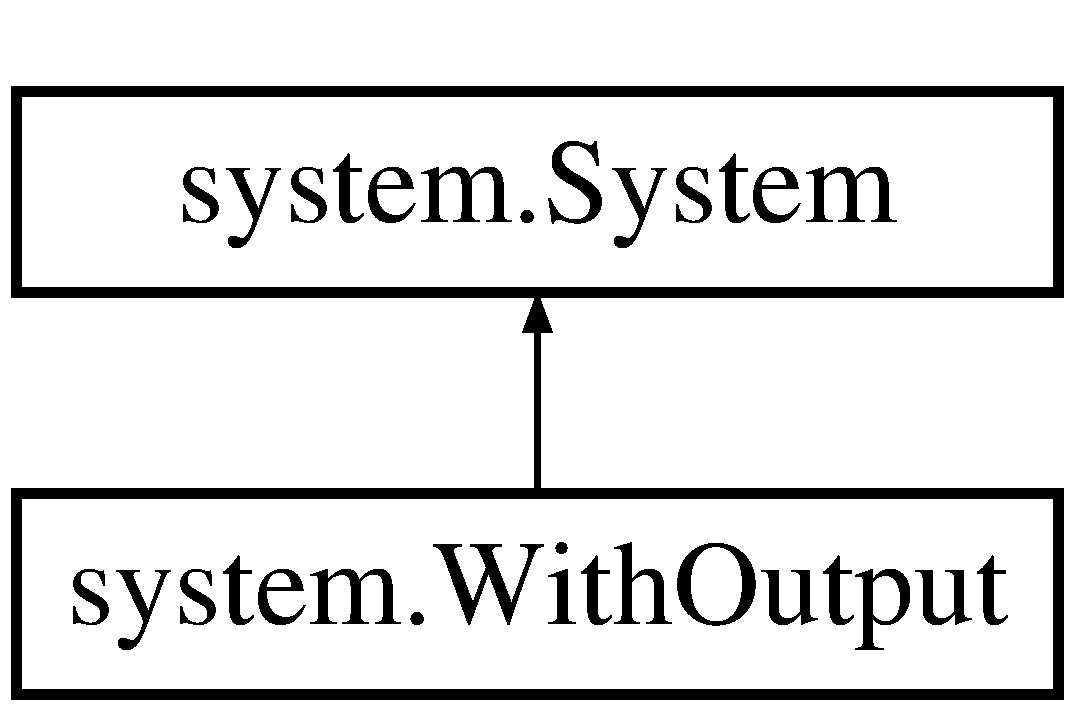
\includegraphics[height=2.000000cm]{d3/dd9/classsystem_1_1System}
\end{center}
\end{figure}
\subsection*{Public Member Functions}
\begin{DoxyCompactItemize}
\item 
def \hyperlink{classsystem_1_1System_ab84763a8a2fcb9acb23ac66607f426ec}{\-\_\-\-\_\-init\-\_\-\-\_\-}
\begin{DoxyCompactList}\small\item\em Initializes a '\hyperlink{classsystem_1_1System}{System}'-\/object. \end{DoxyCompactList}\item 
def \hyperlink{classsystem_1_1System_a9ec2f5b1ad6c228001c7f95cc47446a8}{jump\-\_\-to\-\_\-next\-\_\-event}
\item 
def \hyperlink{classsystem_1_1System_a41d4bfe3fd30910f8d92b5bf182d862e}{run}
\begin{DoxyCompactList}\small\item\em Run the simulation until system time self.\-t exceeds t\-\_\-end. \end{DoxyCompactList}\item 
def \hyperlink{classsystem_1_1System_ad02e76750219966d321e5617e7408e28}{h}
\begin{DoxyCompactList}\small\item\em Update phases according to function H\-\_\-epsilon(phi) as in 'How chaotic is the balanced state' by Jahnke, Memmesheimer and Timme. \end{DoxyCompactList}\item 
def \hyperlink{classsystem_1_1System_a5d42184d0107e6c6777ebde19ff2aa8c}{epsilon}
\begin{DoxyCompactList}\small\item\em Gets the change of the potential for each neuron caused by internal spikes. \end{DoxyCompactList}\item 
def \hyperlink{classsystem_1_1System_a13682705bf8c3b30abb55ee89fe47e96}{get\-\_\-\-Inter\-Spike\-Interval}
\begin{DoxyCompactList}\small\item\em Draws a random inter-\/spike interval according to given rate, and already adds it up to current system time. \end{DoxyCompactList}\item 
def \hyperlink{classsystem_1_1System_aa50493e5779fb6d1e3432be1e2f65605}{get\-\_\-initial\-\_\-\-I\-S\-I}
\item 
def \hyperlink{classsystem_1_1System_a91032897c3c698801333653415cc1c73}{create\-\_\-phases}
\item 
def \hyperlink{classsystem_1_1System_aed8b22289b24b4c09dcf34911f4645b5}{create\-\_\-ext\-\_\-weight\-\_\-matrix}
\item 
def \hyperlink{classsystem_1_1System_a3b3aaa44cf6a8a579e94c7902bbb6473}{create\-\_\-weight\-\_\-matrix}
\end{DoxyCompactItemize}
\subsection*{Public Attributes}
\begin{DoxyCompactItemize}
\item 
\hypertarget{classsystem_1_1System_a9634dee6b17c69008cd4d541a0b3804e}{{\bfseries N}}\label{classsystem_1_1System_a9634dee6b17c69008cd4d541a0b3804e}

\item 
\hypertarget{classsystem_1_1System_a11da6bee25d85cd983c090bfaa7e6eeb}{{\bfseries N\-\_\-ext}}\label{classsystem_1_1System_a11da6bee25d85cd983c090bfaa7e6eeb}

\item 
\hypertarget{classsystem_1_1System_a97d1891bb9376b50b453bf9dc7fa5ef1}{{\bfseries tau}}\label{classsystem_1_1System_a97d1891bb9376b50b453bf9dc7fa5ef1}

\item 
\hyperlink{classsystem_1_1System_ab8fd44fd0fd689735185e83099511489}{I\-\_\-gamma}
\begin{DoxyCompactList}\small\item\em Holds an array of size N (total number of neurons) containing paraters I and gamma for each neuron. \end{DoxyCompactList}\item 
\hypertarget{classsystem_1_1System_ac3d311be1a233827da08d861f1ce798c}{{\bfseries t}}\label{classsystem_1_1System_ac3d311be1a233827da08d861f1ce798c}

\item 
\hypertarget{classsystem_1_1System_a31b7f9e8ccb53a6eab555bfd8ae2af12}{{\bfseries events}}\label{classsystem_1_1System_a31b7f9e8ccb53a6eab555bfd8ae2af12}

\item 
\hypertarget{classsystem_1_1System_adaa4adc9bda791e92e7b349a8d16e333}{\hyperlink{classsystem_1_1System_adaa4adc9bda791e92e7b349a8d16e333}{rates}}\label{classsystem_1_1System_adaa4adc9bda791e92e7b349a8d16e333}

\begin{DoxyCompactList}\small\item\em one rate value per external population \end{DoxyCompactList}\item 
\hypertarget{classsystem_1_1System_a049f8551f240a0b4efd269ec4fb3c425}{\hyperlink{classsystem_1_1System_a049f8551f240a0b4efd269ec4fb3c425}{external\-\_\-events}}\label{classsystem_1_1System_a049f8551f240a0b4efd269ec4fb3c425}

\begin{DoxyCompactList}\small\item\em for each external neuron, holds the (arrival) time of its next spike \end{DoxyCompactList}\item 
\hypertarget{classsystem_1_1System_a58019b9eea1cd90c7a53c5c834fdcf3f}{\hyperlink{classsystem_1_1System_a58019b9eea1cd90c7a53c5c834fdcf3f}{weight\-\_\-matrix}}\label{classsystem_1_1System_a58019b9eea1cd90c7a53c5c834fdcf3f}

\begin{DoxyCompactList}\small\item\em weight matrix, representing the connections and their strengths from any neuron to any other neuron \end{DoxyCompactList}\item 
\hyperlink{classsystem_1_1System_acb0b0396cccf92c3cd63c17b14660490}{phases}
\begin{DoxyCompactList}\small\item\em set dt (time to next event) to a random too large value ... \end{DoxyCompactList}\end{DoxyCompactItemize}


\subsection{Detailed Description}
\begin{DoxyVerb}System of one or more populations of leaky integrate and fire neurons.
Neurons share the same statistical properties among one population; they are modeled as leaky integrate and fire neurons in phase representation as in 'How chaotic is the balanced state' by Jahnke, Memmesheimer and Timme.
\end{DoxyVerb}
 

\subsection{Constructor \& Destructor Documentation}
\hypertarget{classsystem_1_1System_ab84763a8a2fcb9acb23ac66607f426ec}{\index{system\-::\-System@{system\-::\-System}!\-\_\-\-\_\-init\-\_\-\-\_\-@{\-\_\-\-\_\-init\-\_\-\-\_\-}}
\index{\-\_\-\-\_\-init\-\_\-\-\_\-@{\-\_\-\-\_\-init\-\_\-\-\_\-}!system::System@{system\-::\-System}}
\subsubsection[{\-\_\-\-\_\-init\-\_\-\-\_\-}]{\setlength{\rightskip}{0pt plus 5cm}def system.\-System.\-\_\-\-\_\-init\-\_\-\-\_\- (
\begin{DoxyParamCaption}
\item[{}]{self, }
\item[{}]{N = {\ttfamily np.array(\mbox{[}400,100\mbox{]}}, }
\item[{}]{J\-\_\-int = {\ttfamily None}, }
\item[{}]{I = {\ttfamily \mbox{[}1.}, }
\item[{}]{gamma = {\ttfamily \mbox{[}0.2}, }
\item[{}]{K = {\ttfamily 80}, }
\item[{}]{tau = {\ttfamily 0.05}, }
\item[{}]{N\-\_\-ext = {\ttfamily \mbox{[}\mbox{]}}, }
\item[{}]{J\-\_\-ext = {\ttfamily np.array(\mbox{[}\mbox{]})}, }
\item[{}]{rates = {\ttfamily \mbox{[}\mbox{]}}}
\end{DoxyParamCaption}
)}}\label{classsystem_1_1System_ab84763a8a2fcb9acb23ac66607f426ec}


Initializes a '\hyperlink{classsystem_1_1System}{System}'-\/object. 


\begin{DoxyParams}{Parameters}
{\em N} & One-\/dimensional array or list containing the number of individual neurons for each population. \\
\hline
{\em l} & List of firing rates of external inputs (one constant rate per external population/source). \\
\hline
{\em J\-\_\-int} & Two-\/dimensional array containing connection strengths J\-\_\-int\mbox{[}k,l\mbox{]} for connections of neurons from population l to neurons of population k. \\
\hline
{\em J\-\_\-ext} & Two-\/dimensional array containing connection strengths J\-\_\-ext\mbox{[}k,m\mbox{]} for connections from external source m to neurons of population k. \\
\hline
{\em I} & List containing parameters (currents, one value per population) defining properties of the leaky integrate and fire neurons. \\
\hline
{\em gamma} & List containing parameters (leak-\/factor?, one value per population) defining properties of the leaky integrate and fire neurons. \\
\hline
{\em K} & Average number of connections all neurons of one population receive from any other population. \\
\hline
{\em tau} & Delay between sending and receiving an (internal) spike. \\
\hline
\end{DoxyParams}


\subsection{Member Function Documentation}
\hypertarget{classsystem_1_1System_aed8b22289b24b4c09dcf34911f4645b5}{\index{system\-::\-System@{system\-::\-System}!create\-\_\-ext\-\_\-weight\-\_\-matrix@{create\-\_\-ext\-\_\-weight\-\_\-matrix}}
\index{create\-\_\-ext\-\_\-weight\-\_\-matrix@{create\-\_\-ext\-\_\-weight\-\_\-matrix}!system::System@{system\-::\-System}}
\subsubsection[{create\-\_\-ext\-\_\-weight\-\_\-matrix}]{\setlength{\rightskip}{0pt plus 5cm}def system.\-System.\-create\-\_\-ext\-\_\-weight\-\_\-matrix (
\begin{DoxyParamCaption}
\item[{}]{self, }
\item[{}]{J\-\_\-ext, }
\item[{}]{K}
\end{DoxyParamCaption}
)}}\label{classsystem_1_1System_aed8b22289b24b4c09dcf34911f4645b5}
\begin{DoxyVerb}Creates the external weight matrix, that is, weight of connections from each external neuron to each internal neuron.

First, a matrix of random values between 0 and 1 of appropriate size is created. Then, depending on K and the resulting probability to have a connection, the values in the random matrix are set either to 1 or 0 (connection or no connection).
The connections' weights are then set according to J_ext.
@param J_ext Array of connection strength, J_ext[j,i] refers to connections from external population i to internal population j.
@param K Average number of connections one neuron receives from neurons from any other population.
@return External weight matrix.
\end{DoxyVerb}
 \hypertarget{classsystem_1_1System_a91032897c3c698801333653415cc1c73}{\index{system\-::\-System@{system\-::\-System}!create\-\_\-phases@{create\-\_\-phases}}
\index{create\-\_\-phases@{create\-\_\-phases}!system::System@{system\-::\-System}}
\subsubsection[{create\-\_\-phases}]{\setlength{\rightskip}{0pt plus 5cm}def system.\-System.\-create\-\_\-phases (
\begin{DoxyParamCaption}
\item[{}]{self}
\end{DoxyParamCaption}
)}}\label{classsystem_1_1System_a91032897c3c698801333653415cc1c73}
\begin{DoxyVerb}Creates an initial random phase for each neuron.
\end{DoxyVerb}
 \hypertarget{classsystem_1_1System_a3b3aaa44cf6a8a579e94c7902bbb6473}{\index{system\-::\-System@{system\-::\-System}!create\-\_\-weight\-\_\-matrix@{create\-\_\-weight\-\_\-matrix}}
\index{create\-\_\-weight\-\_\-matrix@{create\-\_\-weight\-\_\-matrix}!system::System@{system\-::\-System}}
\subsubsection[{create\-\_\-weight\-\_\-matrix}]{\setlength{\rightskip}{0pt plus 5cm}def system.\-System.\-create\-\_\-weight\-\_\-matrix (
\begin{DoxyParamCaption}
\item[{}]{self, }
\item[{}]{J\-\_\-int, }
\item[{}]{K}
\end{DoxyParamCaption}
)}}\label{classsystem_1_1System_a3b3aaa44cf6a8a579e94c7902bbb6473}
\begin{DoxyVerb}Creates the weight matrix, that is, weight of connections from any internal neuron to each internal neuron.

First, a matrix of random values between 0 and 1 of appropriate size is created. Then, depending on K and the resulting probability to have a connection, the values in the random matrix are set either to 1 or 0 (connection or no connection).
The connections' weights are then set according to J_ext.
@param J_ext Array of connection strength, J_ext[j,i] refers to connections from external population i to internal population j.
@param K Average number of connections one neuron receives from neurons from any other population.
@return Weight matrix.
\end{DoxyVerb}
 \hypertarget{classsystem_1_1System_a5d42184d0107e6c6777ebde19ff2aa8c}{\index{system\-::\-System@{system\-::\-System}!epsilon@{epsilon}}
\index{epsilon@{epsilon}!system::System@{system\-::\-System}}
\subsubsection[{epsilon}]{\setlength{\rightskip}{0pt plus 5cm}def system.\-System.\-epsilon (
\begin{DoxyParamCaption}
\item[{}]{self, }
\item[{}]{spike\-\_\-vector}
\end{DoxyParamCaption}
)}}\label{classsystem_1_1System_a5d42184d0107e6c6777ebde19ff2aa8c}


Gets the change of the potential for each neuron caused by internal spikes. 


\begin{DoxyParams}{Parameters}
{\em spike\-\_\-vector} & Vector of spikes; one entry per neuron (=1 if the neuron spikes, =0 if it does not). \\
\hline
\end{DoxyParams}
\begin{DoxyReturn}{Returns}
epsilon=change in potential for each neuron. 
\end{DoxyReturn}
\hypertarget{classsystem_1_1System_aa50493e5779fb6d1e3432be1e2f65605}{\index{system\-::\-System@{system\-::\-System}!get\-\_\-initial\-\_\-\-I\-S\-I@{get\-\_\-initial\-\_\-\-I\-S\-I}}
\index{get\-\_\-initial\-\_\-\-I\-S\-I@{get\-\_\-initial\-\_\-\-I\-S\-I}!system::System@{system\-::\-System}}
\subsubsection[{get\-\_\-initial\-\_\-\-I\-S\-I}]{\setlength{\rightskip}{0pt plus 5cm}def system.\-System.\-get\-\_\-initial\-\_\-\-I\-S\-I (
\begin{DoxyParamCaption}
\item[{}]{self}
\end{DoxyParamCaption}
)}}\label{classsystem_1_1System_aa50493e5779fb6d1e3432be1e2f65605}
\begin{DoxyVerb}Fills self.external_events with initial (arrival) times of each external neurons' spikes.
\end{DoxyVerb}
 \hypertarget{classsystem_1_1System_a13682705bf8c3b30abb55ee89fe47e96}{\index{system\-::\-System@{system\-::\-System}!get\-\_\-\-Inter\-Spike\-Interval@{get\-\_\-\-Inter\-Spike\-Interval}}
\index{get\-\_\-\-Inter\-Spike\-Interval@{get\-\_\-\-Inter\-Spike\-Interval}!system::System@{system\-::\-System}}
\subsubsection[{get\-\_\-\-Inter\-Spike\-Interval}]{\setlength{\rightskip}{0pt plus 5cm}def system.\-System.\-get\-\_\-\-Inter\-Spike\-Interval (
\begin{DoxyParamCaption}
\item[{}]{self, }
\item[{}]{l\-\_\-i}
\end{DoxyParamCaption}
)}}\label{classsystem_1_1System_a13682705bf8c3b30abb55ee89fe47e96}


Draws a random inter-\/spike interval according to given rate, and already adds it up to current system time. 


\begin{DoxyParams}{Parameters}
{\em l\-\_\-i} & Rate of the poissonian firing of the neuron for which the next spiking time is drawn. \\
\hline
\end{DoxyParams}
\begin{DoxyReturn}{Returns}
Time of next spike. 
\end{DoxyReturn}
\hypertarget{classsystem_1_1System_ad02e76750219966d321e5617e7408e28}{\index{system\-::\-System@{system\-::\-System}!h@{h}}
\index{h@{h}!system::System@{system\-::\-System}}
\subsubsection[{h}]{\setlength{\rightskip}{0pt plus 5cm}def system.\-System.\-h (
\begin{DoxyParamCaption}
\item[{}]{self, }
\item[{}]{epsilon}
\end{DoxyParamCaption}
)}}\label{classsystem_1_1System_ad02e76750219966d321e5617e7408e28}


Update phases according to function H\-\_\-epsilon(phi) as in 'How chaotic is the balanced state' by Jahnke, Memmesheimer and Timme. 

\hypertarget{classsystem_1_1System_a9ec2f5b1ad6c228001c7f95cc47446a8}{\index{system\-::\-System@{system\-::\-System}!jump\-\_\-to\-\_\-next\-\_\-event@{jump\-\_\-to\-\_\-next\-\_\-event}}
\index{jump\-\_\-to\-\_\-next\-\_\-event@{jump\-\_\-to\-\_\-next\-\_\-event}!system::System@{system\-::\-System}}
\subsubsection[{jump\-\_\-to\-\_\-next\-\_\-event}]{\setlength{\rightskip}{0pt plus 5cm}def system.\-System.\-jump\-\_\-to\-\_\-next\-\_\-event (
\begin{DoxyParamCaption}
\item[{}]{self}
\end{DoxyParamCaption}
)}}\label{classsystem_1_1System_a9ec2f5b1ad6c228001c7f95cc47446a8}
\begin{DoxyVerb}One step of simulation; searches for and handles the next event.

Checks whether the next event is the arrival of one or more internal/external spikes or the reset and spike of one or more neurons.
Updates system time self.t by the difference dt between current time and the event found to happen next.
\end{DoxyVerb}
 \hypertarget{classsystem_1_1System_a41d4bfe3fd30910f8d92b5bf182d862e}{\index{system\-::\-System@{system\-::\-System}!run@{run}}
\index{run@{run}!system::System@{system\-::\-System}}
\subsubsection[{run}]{\setlength{\rightskip}{0pt plus 5cm}def system.\-System.\-run (
\begin{DoxyParamCaption}
\item[{}]{self, }
\item[{}]{t\-\_\-end = {\ttfamily 1}}
\end{DoxyParamCaption}
)}}\label{classsystem_1_1System_a41d4bfe3fd30910f8d92b5bf182d862e}


Run the simulation until system time self.\-t exceeds t\-\_\-end. 


\begin{DoxyParams}{Parameters}
{\em t\-\_\-end} & Ending time of the run. \\
\hline
\end{DoxyParams}


\subsection{Member Data Documentation}
\hypertarget{classsystem_1_1System_ab8fd44fd0fd689735185e83099511489}{\index{system\-::\-System@{system\-::\-System}!I\-\_\-gamma@{I\-\_\-gamma}}
\index{I\-\_\-gamma@{I\-\_\-gamma}!system::System@{system\-::\-System}}
\subsubsection[{I\-\_\-gamma}]{\setlength{\rightskip}{0pt plus 5cm}system.\-System.\-I\-\_\-gamma}}\label{classsystem_1_1System_ab8fd44fd0fd689735185e83099511489}


Holds an array of size N (total number of neurons) containing paraters I and gamma for each neuron. 

\hypertarget{classsystem_1_1System_acb0b0396cccf92c3cd63c17b14660490}{\index{system\-::\-System@{system\-::\-System}!phases@{phases}}
\index{phases@{phases}!system::System@{system\-::\-System}}
\subsubsection[{phases}]{\setlength{\rightskip}{0pt plus 5cm}system.\-System.\-phases}}\label{classsystem_1_1System_acb0b0396cccf92c3cd63c17b14660490}


set dt (time to next event) to a random too large value ... 

this will only be used for comparison with time to next emission of spike if there are no other (already emitted) spikes to consider at all check for external event 

The documentation for this class was generated from the following file\-:\begin{DoxyCompactItemize}
\item 
system.\-py\end{DoxyCompactItemize}

\hypertarget{classsystem_1_1WithOutput}{\section{system.\-With\-Output Class Reference}
\label{classsystem_1_1WithOutput}\index{system.\-With\-Output@{system.\-With\-Output}}
}
Inheritance diagram for system.\-With\-Output\-:\begin{figure}[H]
\begin{center}
\leavevmode
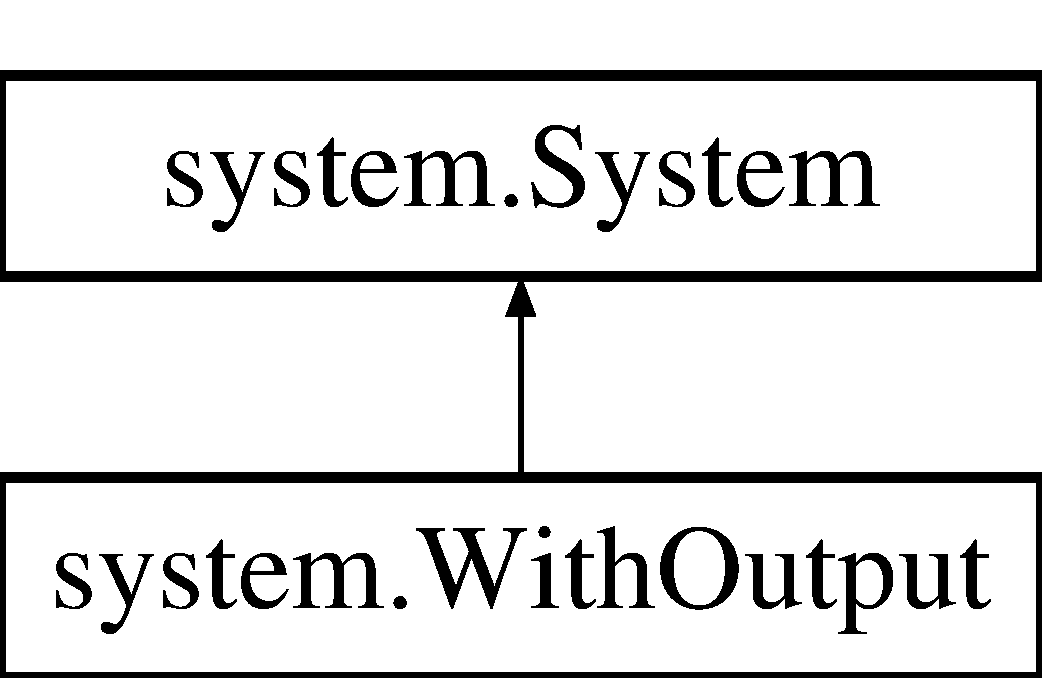
\includegraphics[height=2.000000cm]{dd/d44/classsystem_1_1WithOutput}
\end{center}
\end{figure}
\subsection*{Public Member Functions}
\begin{DoxyCompactItemize}
\item 
def \hyperlink{classsystem_1_1WithOutput_a60b38b97c97568583fc2cf54cb7e8678}{\-\_\-\-\_\-init\-\_\-\-\_\-}
\item 
def \hyperlink{classsystem_1_1WithOutput_abeb008bf9930662467931e61a741b763}{run}
\end{DoxyCompactItemize}
\subsection*{Public Attributes}
\begin{DoxyCompactItemize}
\item 
\hypertarget{classsystem_1_1WithOutput_af6dac20f0117ff620ec5d157ff223377}{{\bfseries parameters}}\label{classsystem_1_1WithOutput_af6dac20f0117ff620ec5d157ff223377}

\item 
\hypertarget{classsystem_1_1WithOutput_a272fee7b8df6177d883f0d257628eeff}{{\bfseries n\-\_\-files}}\label{classsystem_1_1WithOutput_a272fee7b8df6177d883f0d257628eeff}

\item 
\hypertarget{classsystem_1_1WithOutput_adc7afae162437b6c0e4d15434e6ac625}{{\bfseries outputs}}\label{classsystem_1_1WithOutput_adc7afae162437b6c0e4d15434e6ac625}

\end{DoxyCompactItemize}


\subsection{Detailed Description}
\begin{DoxyVerb}WithOutput inherits the class System. It is very similar, but has some functionalities implemented to write data generated during a simulation to an output folder. Furthermore, it displays some more output on the command line when the simulation is running (progress bar).
\end{DoxyVerb}
 

\subsection{Constructor \& Destructor Documentation}
\hypertarget{classsystem_1_1WithOutput_a60b38b97c97568583fc2cf54cb7e8678}{\index{system\-::\-With\-Output@{system\-::\-With\-Output}!\-\_\-\-\_\-init\-\_\-\-\_\-@{\-\_\-\-\_\-init\-\_\-\-\_\-}}
\index{\-\_\-\-\_\-init\-\_\-\-\_\-@{\-\_\-\-\_\-init\-\_\-\-\_\-}!system::WithOutput@{system\-::\-With\-Output}}
\subsubsection[{\-\_\-\-\_\-init\-\_\-\-\_\-}]{\setlength{\rightskip}{0pt plus 5cm}def system.\-With\-Output.\-\_\-\-\_\-init\-\_\-\-\_\- (
\begin{DoxyParamCaption}
\item[{}]{self, }
\item[{}]{N = {\ttfamily np.array(\mbox{[}400,100\mbox{]}}, }
\item[{}]{J\-\_\-int = {\ttfamily np.array(\mbox{[}\mbox{]})}, }
\item[{}]{I = {\ttfamily \mbox{[}1.}, }
\item[{}]{gamma = {\ttfamily \mbox{[}0.2}, }
\item[{}]{K = {\ttfamily 50}, }
\item[{}]{tau = {\ttfamily 0.05}, }
\item[{}]{N\-\_\-ext = {\ttfamily \mbox{[}\mbox{]}}, }
\item[{}]{J\-\_\-ext = {\ttfamily np.array(\mbox{[}\mbox{]})}, }
\item[{}]{rates = {\ttfamily \mbox{[}\mbox{]}}}
\end{DoxyParamCaption}
)}}\label{classsystem_1_1WithOutput_a60b38b97c97568583fc2cf54cb7e8678}
\begin{DoxyVerb}Initializes a 'WithOutput'-object.
@param N One-dimensional array or list containing the number of individual neurons for each population.
@param l List of firing rates of external inputs (one constant rate per external population/source).
@param J_int Two-dimensional array containing connection strengths J_int[k,l] for connections of neurons from population l to neurons of population k.
@param J_ext Two-dimensional array containing connection strengths J_ext[k,m] for connections from external source m to neurons of population k.
@param I List containing parameters (currents, one value per population) defining properties of the leaky integrate and fire neurons.
@param gamma List containing parameters (leak-factor?, one value per population) defining properties of the leaky integrate and fire neurons.
@param K Average number of connections all neurons of one population receive from any other population.
@param tau Delay between sending and receiving an (internal) spike.
\end{DoxyVerb}
 

\subsection{Member Function Documentation}
\hypertarget{classsystem_1_1WithOutput_abeb008bf9930662467931e61a741b763}{\index{system\-::\-With\-Output@{system\-::\-With\-Output}!run@{run}}
\index{run@{run}!system::WithOutput@{system\-::\-With\-Output}}
\subsubsection[{run}]{\setlength{\rightskip}{0pt plus 5cm}def system.\-With\-Output.\-run (
\begin{DoxyParamCaption}
\item[{}]{self, }
\item[{}]{t\-\_\-end, }
\item[{}]{output\-\_\-dir}
\end{DoxyParamCaption}
)}}\label{classsystem_1_1WithOutput_abeb008bf9930662467931e61a741b763}
\begin{DoxyVerb}Run the simulation until system time self.t exceeds t_end, creates folder output_dir and writes output to it.
@param t_end Ending time of the run.
@param output_dir A string specifying the folder to which the output should be written.
\end{DoxyVerb}
 

The documentation for this class was generated from the following file\-:\begin{DoxyCompactItemize}
\item 
system.\-py\end{DoxyCompactItemize}

%--- End generated contents ---

% Index
\newpage
\phantomsection
\addcontentsline{toc}{chapter}{Index}
\printindex

\end{document}
